
\section{Informal specifications}
\label{sec:informal-specification}

Before we provide an informal specification of \peek and \poke, respectively,
we introduce some auxiliary concepts and formulate general assumptions.
We would also like to point out the following: 
When we speak of \emph{integers}, then we refer to the infinite set of mathematical
integers $\{\ldots, -1, 0, 1, \ldots\}$
and not to one of the many finite representation provided by the type system of~C.
This distinction is important because mathematical integers
usually play an important role in \acsl specifications.

\subsection{Basic concepts}

\begin{itemize}
\item
A \emph{bit stream} is an array containing elements of type \verb"uint8_t".

A bit stream of length $n$ contains $8n$ bits.

\item
A bit stream is \emph{valid} if the array is valid.

\item 
A bit stream can be indexed both by its array indices
and its \emph{bit indices}.

Figure~\ref{fig:bitstream-indices} shows the difference between 
array indices and bit indices in a bit stream.
The two bit indices, 0~and~14,
mark bit positions in the first and second array element, respectively.

\begin{figure}[hbt]
\begin{center}
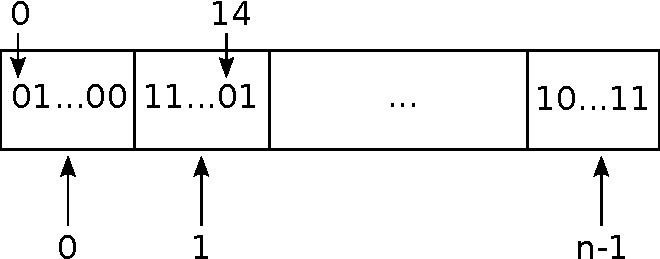
\includegraphics[width=0.40\textwidth]{figures/array_as_stream.pdf}
\caption{\label{fig:bitstream-indices} Array indices and bit indices in a bit stream}
\end{center}
\end{figure}

\item 
The C~programming language neither provides a type \emph{bit}
nor does it support random access to the bits of a bit stream.
In order to access the $i$-th bit of a bit sequence one typically
has to first access the byte with index $j = i/8$ and then access the 
bit $k = i \pmod{8}$ within this byte.
Note that in Figure~\ref{fig:bitstream-indices} 
bytes and bits are indexed in increasing order from the \emph{left}.
On the byte level, however, bits are often indexed from the \emph{right}.
For example, to access the $k$-th bit of a byte \inl{a} one can
shift this bit to the right by $7-k$ and extracts then the now
rightmost bit by performing a bit-wise \emph{and} with the value~1
%
\begin{verbatim}
   (a >> (7-k)) & 1
\end{verbatim}

\item
A \emph{bit sequence} is a consecutive sequence of bits within a bit stream
as represented in Figure~\ref{fig:bitsequence}.
\begin{figure}[hbt]
\begin{center}
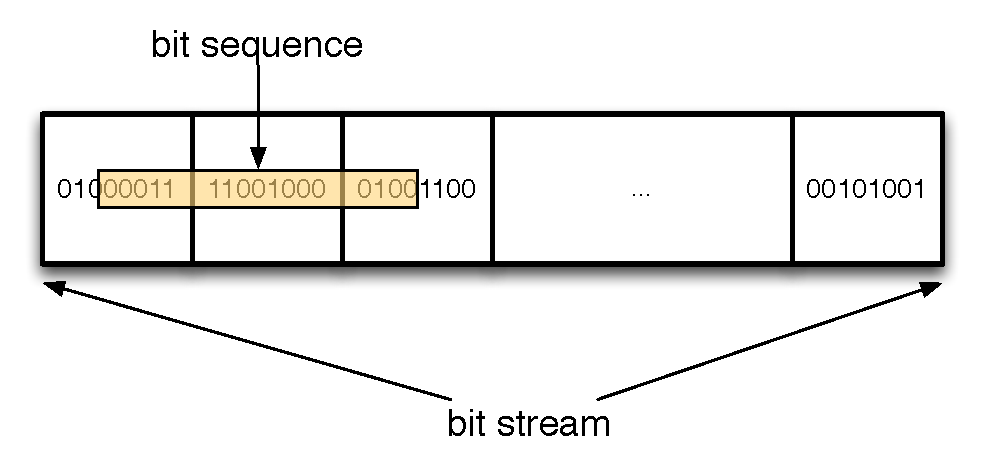
\includegraphics[width=0.40\textwidth]{figures/bit_sequence.pdf}
\caption{\label{fig:bitsequence} A bit sequence within a bit stream}
\end{center}
\end{figure}

A bit sequence is given by the position of its first bit (a bit index in the bit stream)
and its \emph{length}, that is, the number of bits it contains.

\item A bit sequence of length $l$ that starts at bit index $p$ is \emph{valid}
     with respect to a bit stream of length $n$ if the following conditions are
     satisfied
     \begin{align*}
         0 &\leq p < 8n \\
         0 &\leq p + l < 8n
     \end{align*}

\end{itemize}

We assume that the C-types \inl{unsigned int} and \inl{int}, which
are used in the implementation to represent indices, counting and error codes,
have a width of~32~bits.
We point this out here because we conducted the verification on a platform with
these characteristics.

As an aside, MISRA-C discourages the use of ``generic'' integer types
such as \inl{int} and \inl{unsigned int} and recommends the use of integer types whose names
contain the exact width.

\subsection{Informal specification of \peek}
\label{sec:informal-peek}

Now we specify \peek with the introduced auxiliary concepts.
The function \peek reads a bit sequence from a bit stream
and converts it to an integer.

Its function signature reads as follows:

\begin{lstlisting}[style=acsl-block]
uint64_t  Bitwalker_Peek(unsigned int Startposition, 
                         unsigned int Length,
                         uint8_t Bitstream[],
                         unsigned int BitstreamSizeInBytes);
\end{lstlisting}

\paragraph{Arguments}
The arguments of \peek have the following purpose:
\begin{itemize}
    \item \inl{Startposition} is the bit index in the bit stream 
    where the bit sequence starts.
    \item \inl{Length} is the length of the bit sequence.
    \item \inl{Bitstream} is the array which provides the bit stream.
    \item \inl{BitstreamSizeInBytes} is the length of the array 
    containing the bit stream. 
\end{itemize}

\paragraph{Preconditions}
The following preconditions shall hold for the function arguments.
Note that additional constraints are implicitly expressed by the use
of \emph{unsigned} integer types.

\begin{itemize}
\item \inl{Bitstream} is a valid array of length \inl{BitstreamSizeInBytes}

\item \inl{Length} $\leq$ \inl{64} and

\item \inl{Startposition} $\leq$ \inl{UINT_MAX} - \inl{Length}.
      This condition expresses that no arithmetic overflows shall occur
      when evaluating \inl{Startposition + Length}.
\end{itemize}

\paragraph{Description}
As mentioned, the function \peek reads a bit sequence from a bit stream
and converts it to a 64-bit unsigned integer.

For a bit sequence $(b_0, b_1,\ldots,b_{n - 1})$ the function \peek returns the sum
\begin{align}
\label{eq:peek-result}
    \sum_{i=0}^{n-1} b_i \cdot 2^{(n - 1) - i} 
\end{align}

Note that is a higher-level description than what is done in the source code.
There is, in our opinion, not much point to reflect all of the low-level bit operations
into the specification if a clearer description is at hand.

If the bit sequence is not valid, then \peek shall return~0.
We were wondering why the implementation maps an illegal input to a legitimate output.
The code providers argued along the lines that this error condition was not
considered important enough to be properly reported.
One can interpret this design decision as an attempt to increase the
robustness of the function against illegal values.
In general, we recommend to explicitly describe all error conditions
and to devise a consistent error detection and error recovery strategy.


\subsection{Informal specification of \poke}
\label{sec:informal-poke}

In this section we examine the function \poke
in the same manner as we did it for \peek.

The function \poke converts an integer to a bit sequence and writes it
into a bit stream.
Its function signature reads as follows:
\begin{lstlisting}[style = acsl-block]
int      Bitwalker_Poke(unsigned int Startposition,
                        unsigned int Length,
                        uint8_t Bitstream[],
                        unsigned int BitstreamSizeInBytes,
                        uint64_t Value);
\end{lstlisting}


\paragraph{Arguments}
The arguments have the following purpose:

\begin{itemize}
    \item \inl{Startposition} is the bit index in the bit stream 
    where the bit sequence starts.
    \item \inl{Length} is the length of the bit sequence.
    \item \inl{Bitstream} is the array which provides the bit stream.
    \item \inl{BitstreamSizeInBytes} is the length of the array 
    containing the bit stream. 
    \item \inl{Value} is the integer which shall be converted into a bit sequence.
\end{itemize}


\paragraph{Preconditions}
The following conditions shall hold for the function arguments:

\begin{itemize}
\item \inl{Bitstream} is a valid array of length \inl{BitstreamSizeInBytes}

\item \inl{Startposition + Length} is less than \verb"UINT_MAX".
\end{itemize}

Note that additional constraints are implicitly expressed by the use
of \emph{unsigned} integer types.


\paragraph{Description}
Now we can specify \poke as follows:
The function \poke converts a 64-bit unsigned integer to a bit sequence and 
writes it into a bit stream.

For $0 \leq x$ exists a shortest sequence of~0 and~1
$(b_0, b_1,\ldots,b_{n - 1})$
such that
\begin{align}
    \sum_{i=0}^{n-1} b_i \cdot 2^{(n - 1) - i} = x.
\end{align}

The function \poke tries to store the sequence $(b_0, b_1,\ldots,b_{n - 1})$
in the bit sequence of \inl{Length} bits that starts
at bit index \inl{Startposition}.

The return value of \poke depends on the following three cases:

\begin{itemize}
\item 
If the bit sequence is not valid, then \poke returns~$-1$.

\item 
If the bit sequence is valid, then there are two cases:

\begin{itemize}
\item
If $x$ is greater or equal than $2^\mathtt{Length}$, then~$x$
cannot be represented as bit sequence $(b_0, b_1,\ldots,b_{\mathtt{Length} - 1})$.
\poke returns then~$-2$.

\item
If $x$ is less the $2^{\mathtt{Length}}$, then  the sequence
$(\overbrace{0,\ldots,0}^{\mathtt{Length}-n},b_0, b_1,\ldots,b_{n - 1})$
is stored in the bit stream starting at \inl{Startposition}.
The return value of \poke is 0.

\end{itemize}
\end{itemize}

